\documentclass[10pt,conference,a4paper]{IEEEtran}
\usepackage[utf8]{inputenc}
\usepackage{graphicx}
\usepackage{float}
\usepackage{enumerate}
\usepackage[spanish]{babel}
\usepackage[hidelinks]{hyperref}

%opening
\title{[ELO313] Procesamiento Digital de Se\~nales\\ 
Tarea I}
\author{Cristian Acuña S.{\small $~^1$}
\vspace{1.6mm}\\
Departamento de Electrónica, Universidad Técnica Federico Santa María.\\
	Avenida España 1680, Valparaíso, Chile.\\
	\fontsize{9}{9}\selectfont\ttfamily\upshape

	$~^{1}$\,cristian.acuna@alumnos.usm.cl (2921006-3)
}
\date{6 de Mayo de 2014}

\begin{document}

\maketitle

\section{Evaluaci\'on de Propiedades de Sistemas}

Se pide verificar las propiedades de invariancia en el tiempo, linealidad y 
causalidad para ciertos sistemas desconocidos \verb|bbox1|, \verb|bbox2| y 
\verb|bbox3|.

\subsection{Invariancia en el tiempo}

Para probar esta propiedad, los sistemas son estimulados con pulso cuadrado de 
largo total 30 ($\mu[n-10]-\mu[n-20]$), y luego estimulados con la misma 
se\~nal con un retraso temporal ($\mu[n-15]-\mu[n-25]$). Para dichos sistemas, 
se presentan los resultados de estos est\'imulos en las figuras 
(\ref{fig:img1}), (\ref{fig:img2}) y (\ref{fig:img3}) respectivamente.

\begin{figure}[H]
  \centering
  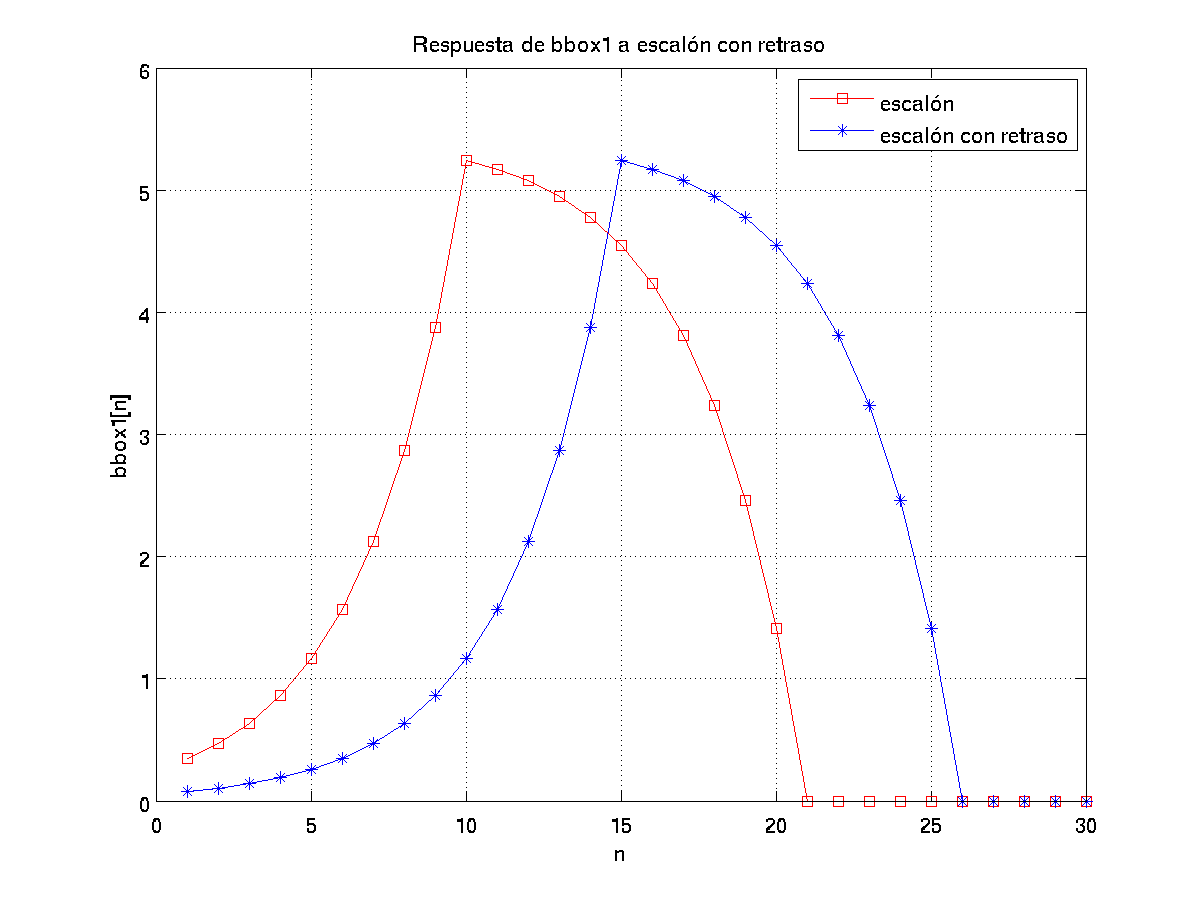
\includegraphics[width=0.45\textwidth]{../img/img1.png}
  \caption{Respuesta de bbox1.}
  \label{fig:img1}
\end{figure}

\begin{figure}[H]
  \centering
  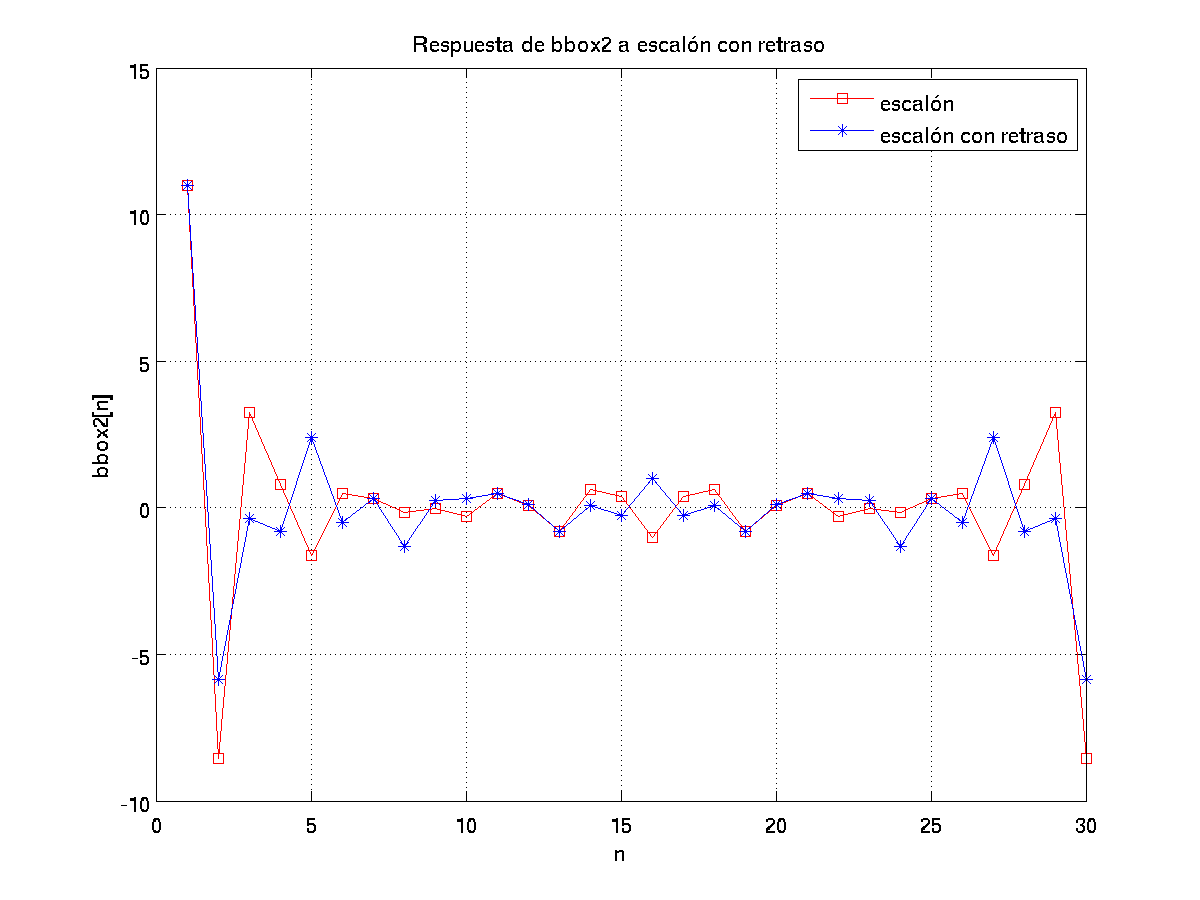
\includegraphics[width=0.45\textwidth]{../img/img2.png}
  \caption{Respuesta de bbox2.}
  \label{fig:img2}
\end{figure}

\begin{figure}[H]
  \centering
  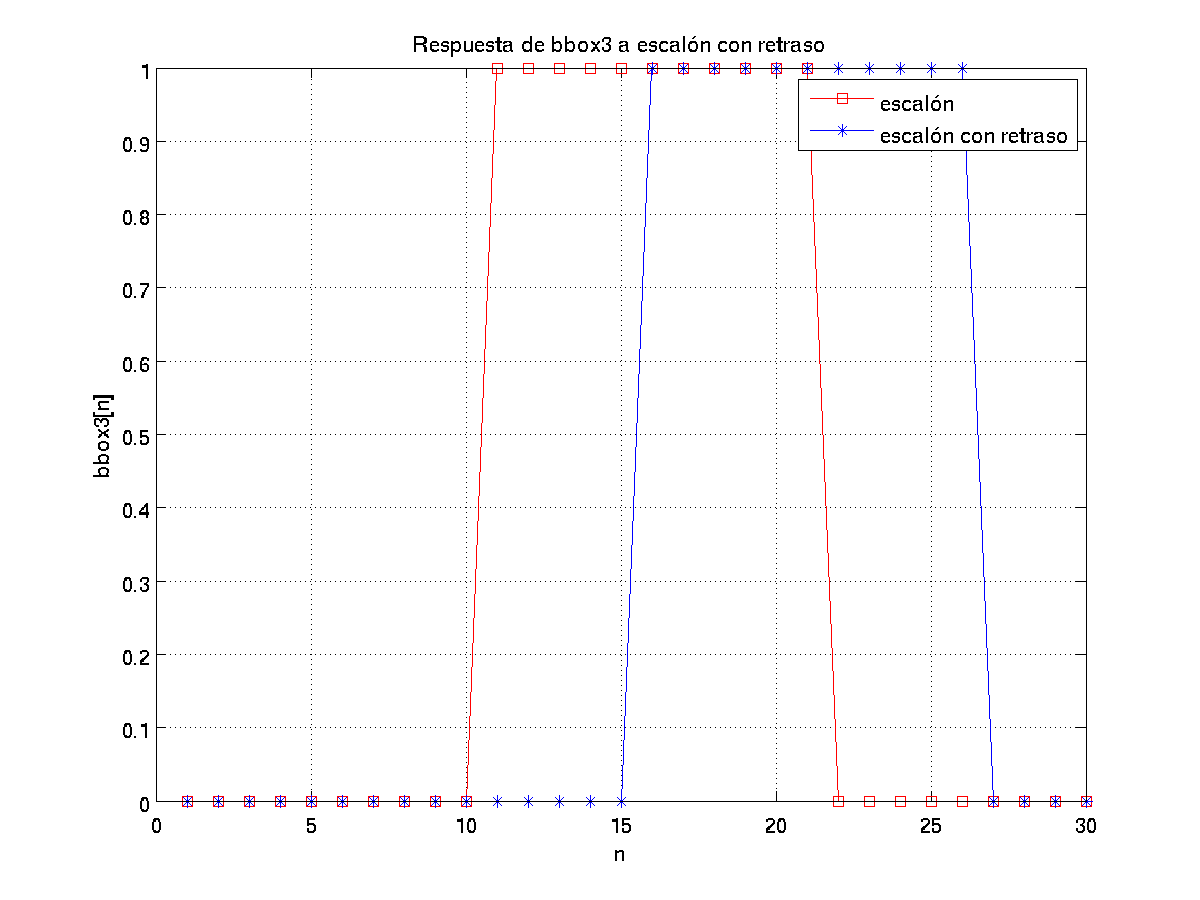
\includegraphics[width=0.45\textwidth]{../img/img3.png}
  \caption{Respuesta de bbox3.}
  \label{fig:img3}
\end{figure}

Se puede apreciar en la figura (\ref{fig:img2}) que la respuesta de \verb|bbox2|
ante una se\~nal no es la misma se\~nal retrasada. En este caso corresponde a 
una se\~nal diferente. Por lo tanto, se puede concluir que \verb|bbox2| es un 
sistema que var\'ia con el tiempo.

\subsection{Linealidad}

Para probar esta propiedad, cada sistema es excitado a dos se\~nales, un pulso 
cuadrado (igual al punto anterior) y a una sinusoide. Luego, se comparan las 
respuestas por separado sumadas con la respuesta del sistema en cuesti\'on a la 
suma de ambas se\~nales. Si se cumple linealidad, ambos gr\'aficos debiesen ser 
iguales. De otro modo, se puede decir que dicho sistema es \emph{no-lineal}.
Para dichos sistemas, se presenta el resultado de dichos experimentos en las 
figuras (\ref{fig:img4}), (\ref{fig:img5}) y (\ref{fig:img6}).

\begin{figure}[H]
  \centering
  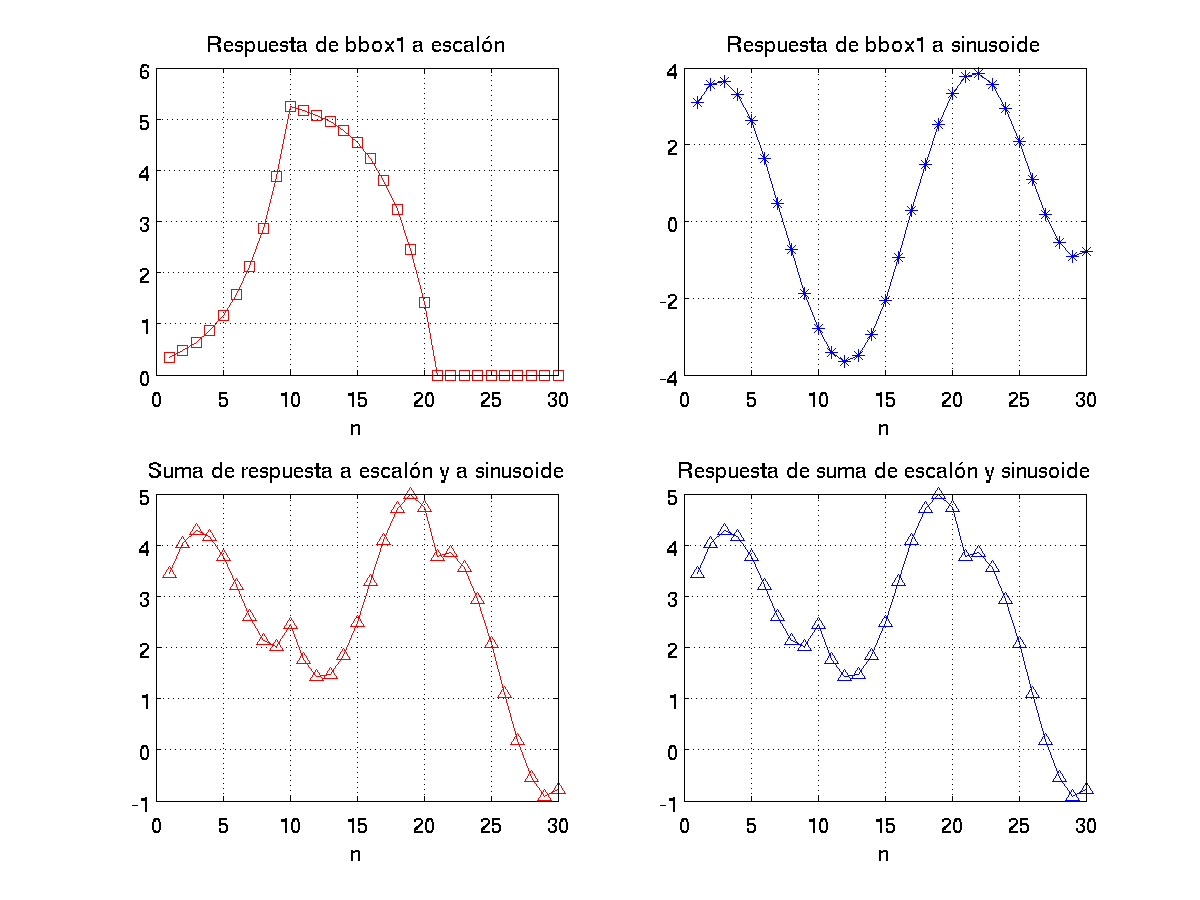
\includegraphics[width=0.45\textwidth]{../img/img4.png}
  \caption{Respuesta de bbox1.}
  \label{fig:img4}
\end{figure}

\begin{figure}[H]
  \centering
  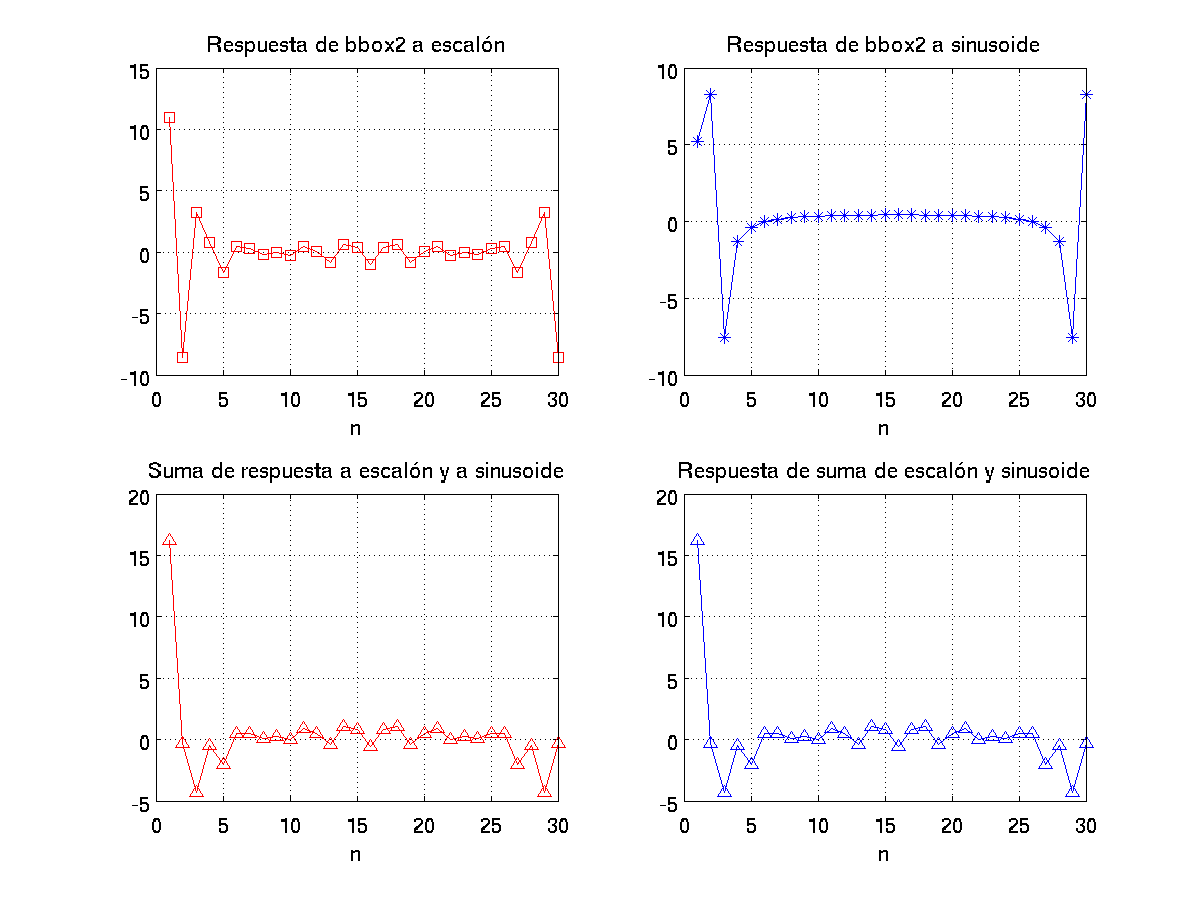
\includegraphics[width=0.45\textwidth]{../img/img5.png}
  \caption{Respuesta de bbox2.}
  \label{fig:img5}
\end{figure}

\begin{figure}[H]
  \centering
  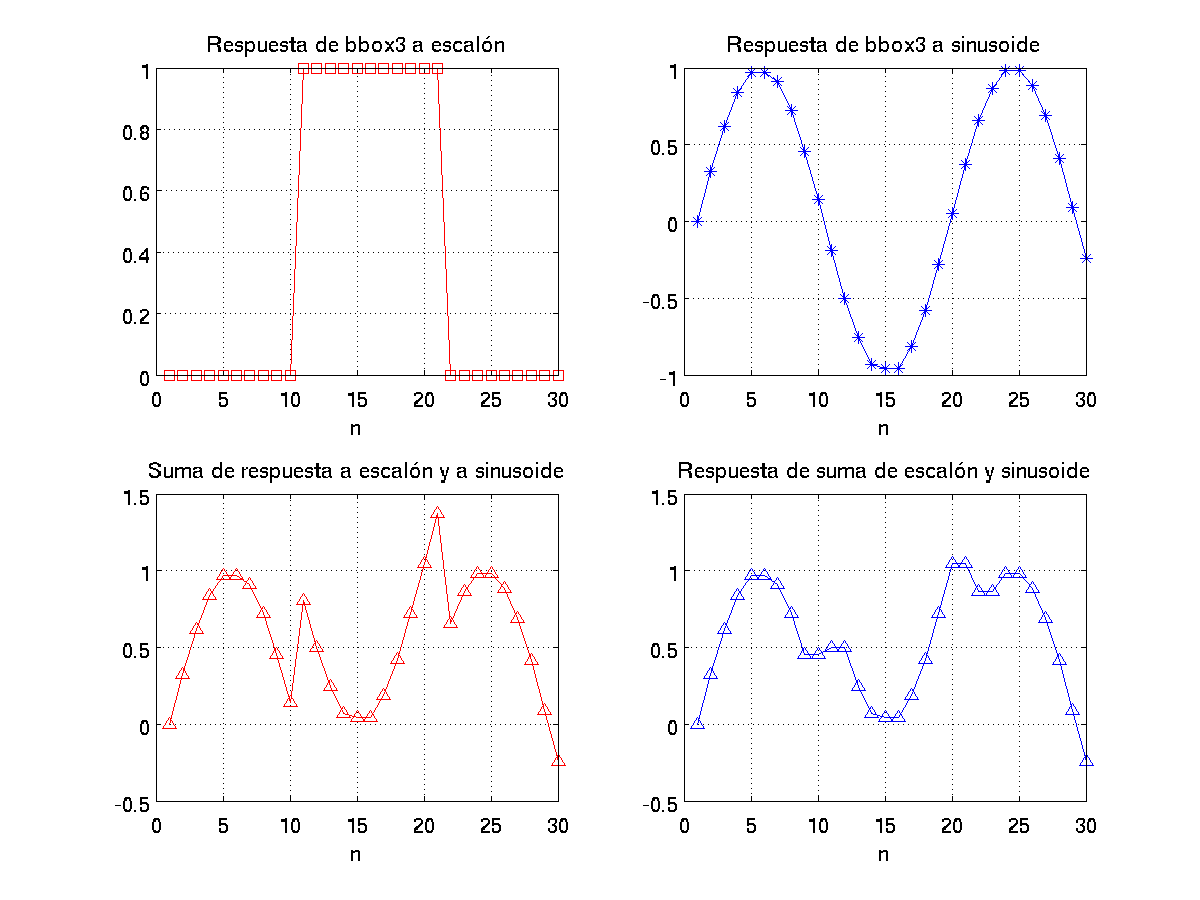
\includegraphics[width=0.45\textwidth]{../img/img6.png}
  \caption{Respuesta de bbox3.}
  \label{fig:img6}
\end{figure}

Por lo tanto, se puede concluir de la figura (\ref{fig:img6}) que el sistema 
\verb|bbox3| es no-lineal.

\subsection{Causalidad y Estabilidad (BIBO)}

Para poder probar la \emph{causalidad} y la \emph{estabilidad} (\emph{BIBO})
de los sistemas entregados, se procede a estimularlos con un impulso discreto 
(Delta de Kr\"onecker) desplazado en el tiempo ($\delta_K(t-14)$). Los 
resultados se muestran en las figuras (\ref{fig:img7}), (\ref{fig:img8}) y 
(\ref{fig:img9}).

\begin{figure}[H]
  \centering
  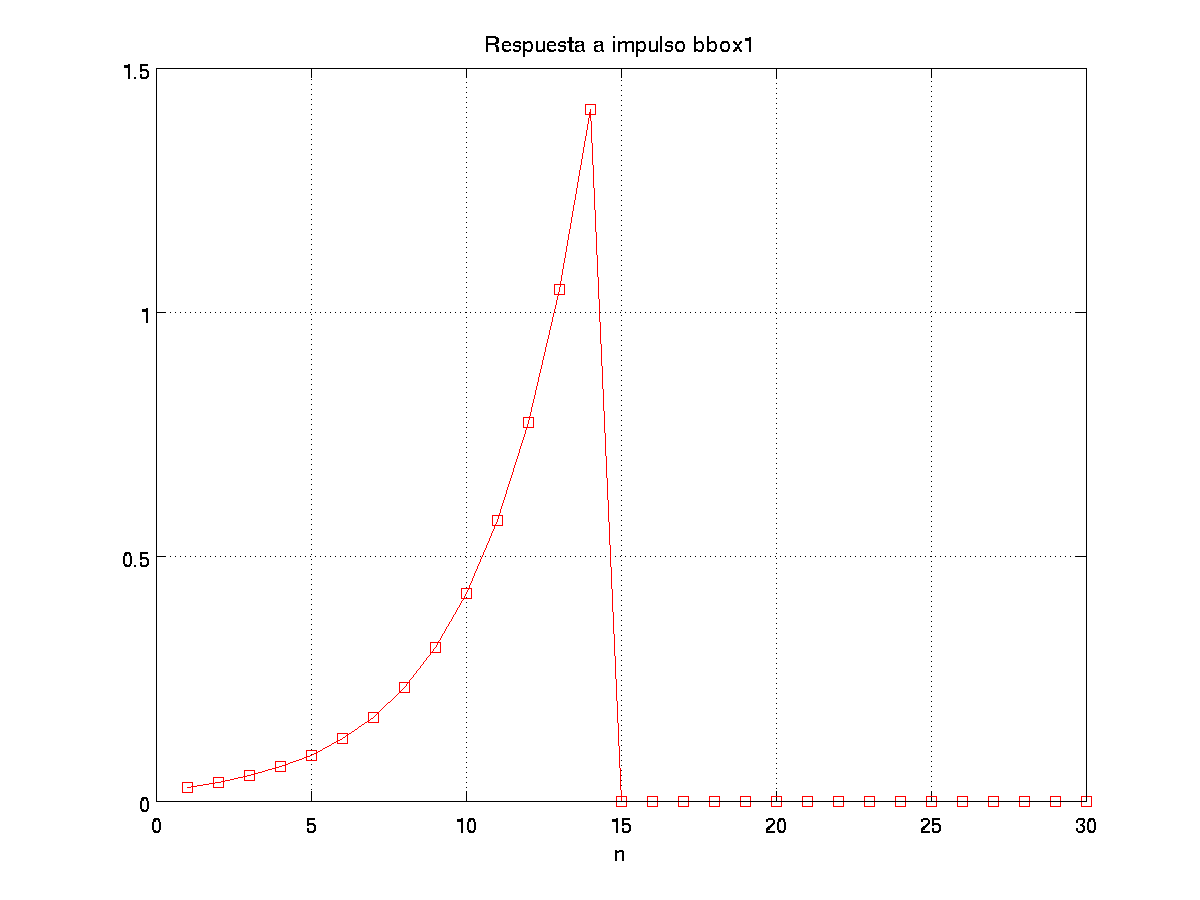
\includegraphics[width=0.45\textwidth]{../img/img7.png}
  \caption{Respuesta de bbox1.}
  \label{fig:img7}
\end{figure}

\begin{figure}[H]
  \centering
  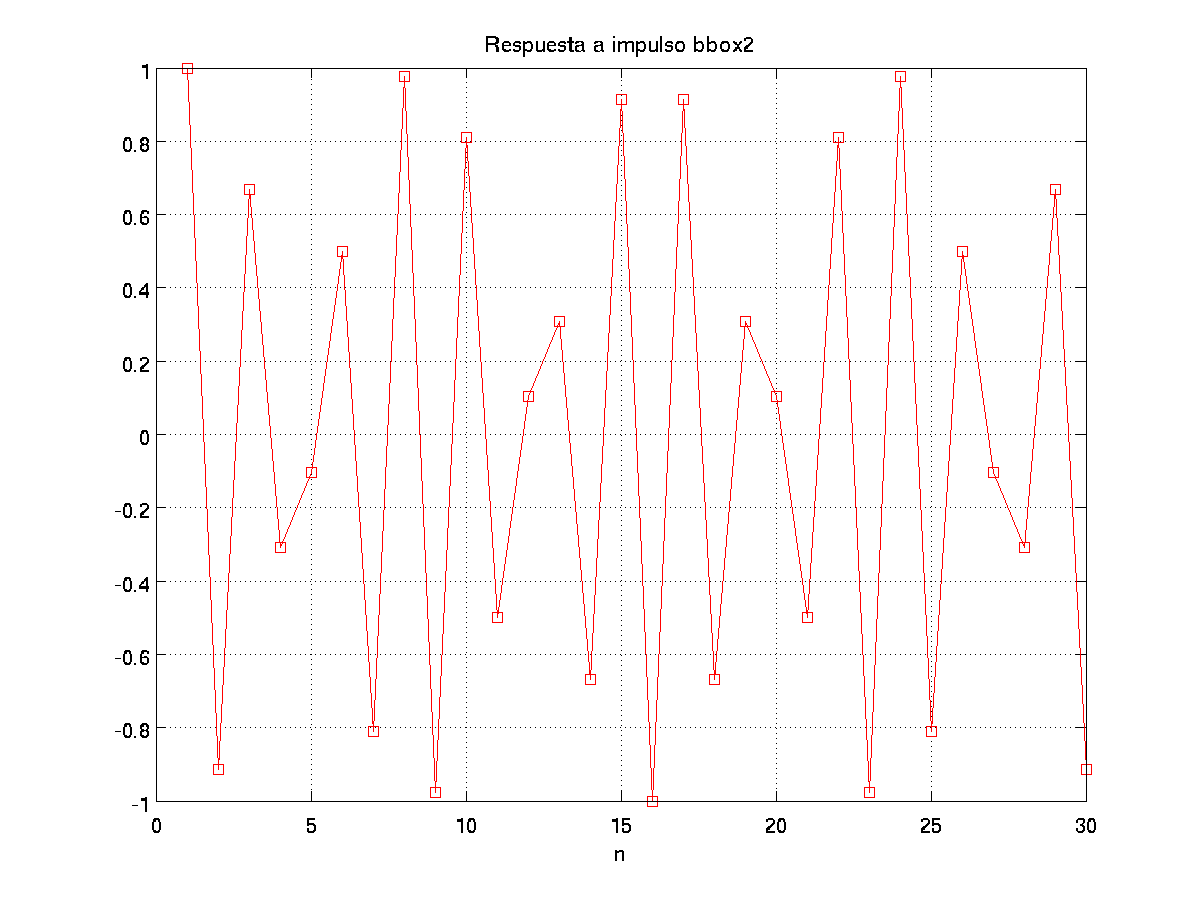
\includegraphics[width=0.45\textwidth]{../img/img8.png}
  \caption{Respuesta de bbox2.}
  \label{fig:img8}
\end{figure}

\begin{figure}[H]
  \centering
  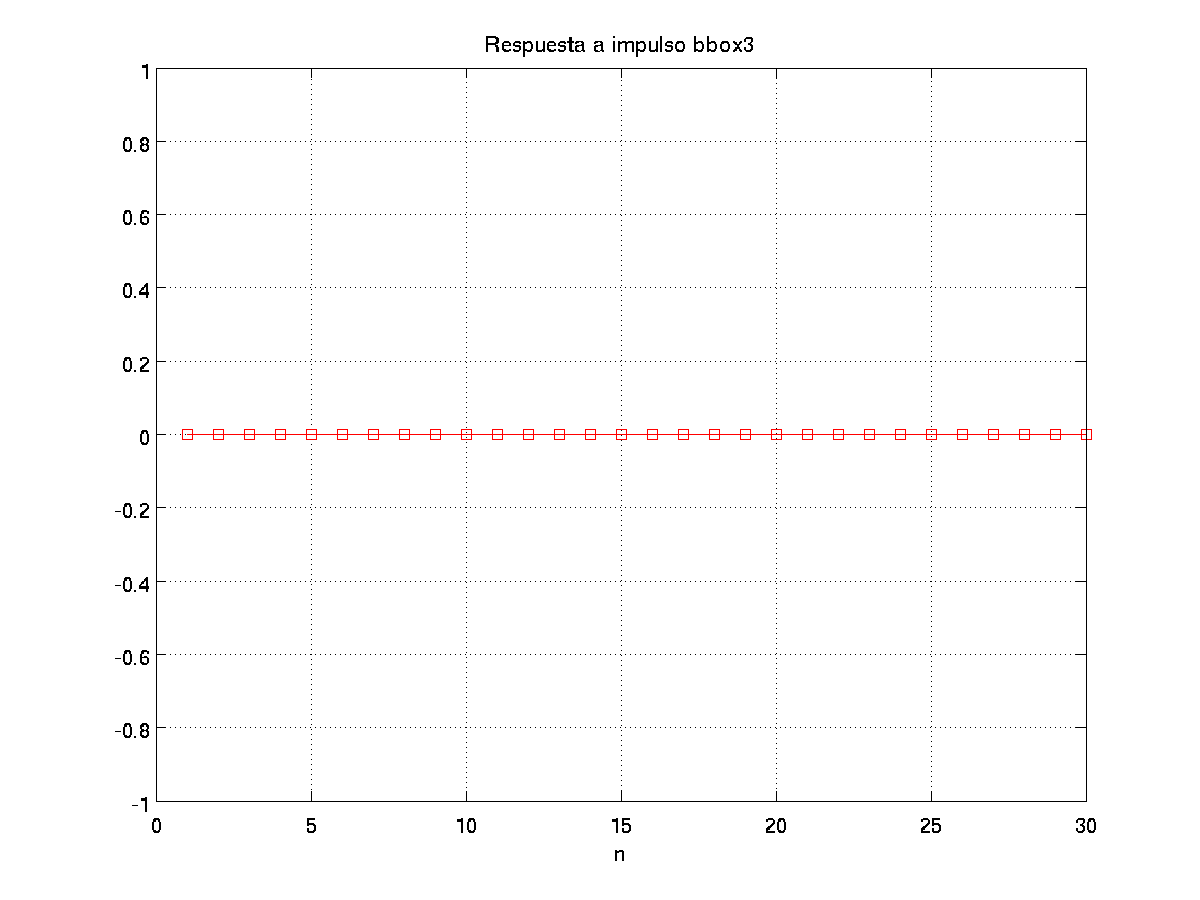
\includegraphics[width=0.45\textwidth]{../img/img9.png}
  \caption{Respuesta de bbox3.}
  \label{fig:img9}
\end{figure}

De las figuras anteriores, se puede concluir:

\begin{itemize}
 \item El sistema \verb|bbox1| presenta respuesta en tiempos anteriores al 
tiempo de exitaci\'on, por lo cual se puede decir que es un sistema 
\textbf{no-causal}. Con respecto a su estabilidad, se puede observar que el 
sistema luego de ser excitado vuelve a su estado de reposo, por lo que es un 
sistema \textbf{estable} seg\'un el criterio BIBO.
 \item El sistema \verb|bbox2| presenta respuesta a excitaci\'on en tiempos 
anteriores al tiempo de excitaci\'on, por lo cual corresponde a un sistema 
\textbf{no-causal}. En cuanto a su estabilidad, es sistema no vuelve al reposo 
luego de ser estimulado, sino que se mantiene excitado, por lo que corresponde 
a un sistema \textbf{inestable}.
 \item El sistema \verb|bbox3| no presenta respuesta en tiempos previos a ser 
excitado, por lo que corresponde a un sistema \textbf{causal}. Adem\'as, el 
sistema no presenta se\~nal luego de ser excitado, por lo que corresponde a un 
sistema \textbf{estable}.
\end{itemize}


\end{document}
